% Fig. 2  Semantic-layer workflow (single column, drawn at 3.45 in).
% Provenance: orchestrator.py step 12b at 78d906b (K1), a63cec1 (K3) and b11793b (fail-closed fix);
% semantics/verify.py: verify_semantics = build_spec -> typecheck -> preserve -> SemanticReport.
\documentclass[border=2pt]{standalone}
% Shared settings for all InsightFlow AI figures (Times, grayscale, sized for IEEE print).
\usepackage[T1]{fontenc}
\usepackage{mathptmx}
\usepackage{tikz}
\usetikzlibrary{positioning,arrows.meta,calc,fit,patterns,shapes.geometric}
\tikzset{
  >={Stealth[length=4pt,width=3.5pt]},
  stage/.style={draw,rounded corners=1.5pt,fill=gray!8,align=center,inner sep=2.5pt,font=\fontsize{7.5}{8.6}\selectfont},
  ext/.style={draw,dashed,rounded corners=1.5pt,align=center,inner sep=2.5pt,font=\fontsize{7.5}{8.6}\selectfont},
  note/.style={align=left,font=\fontsize{7}{8}\selectfont},
  flow/.style={->,thick},
  dflow/.style={->,dashed},
  every node/.append style={execute at begin node={\hyphenpenalty=10000\exhyphenpenalty=10000}},
}

\begin{document}
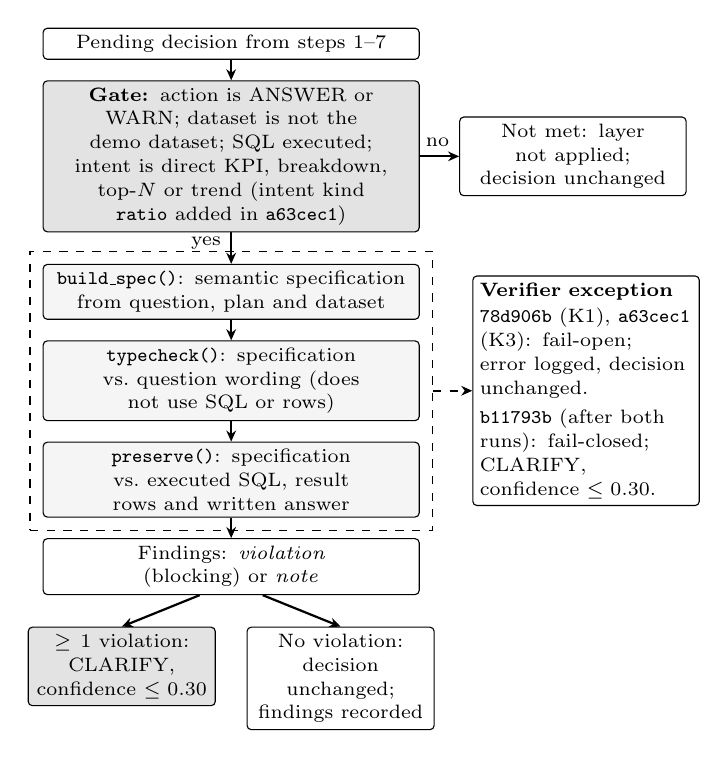
\begin{tikzpicture}[node distance=2.6mm]
  \tikzset{main/.style={stage,text width=46mm}}
  \node[main,fill=white] (in) {Pending decision from steps 1--7};
  \node[main,below=of in,fill=gray!22] (gate) {\textbf{Gate:} action is ANSWER or WARN; dataset is not the demo dataset; SQL executed; intent is direct KPI, breakdown, top-$N$ or trend (intent kind \texttt{ratio} added in \texttt{a63cec1})};
  \node[main,below=4mm of gate] (spec) {\texttt{build\_spec()}: semantic specification from question, plan and dataset};
  \node[main,below=of spec] (tc) {\texttt{typecheck()}: specification vs.\ question wording (does not use SQL or rows)};
  \node[main,below=of tc] (pr) {\texttt{preserve()}: specification vs.\ executed SQL, result rows and written answer};
  \node[main,below=of pr,fill=white] (rep) {Findings: \emph{violation} (blocking) or \emph{note}};
  \node[stage,text width=22mm,below left=4mm and -22mm of rep,fill=gray!22] (clar) {$\ge 1$ violation: CLARIFY, confidence $\le 0.30$};
  \node[stage,text width=22mm,below right=4mm and -22mm of rep,fill=white] (keep) {No violation: decision unchanged; findings recorded};
  \draw[flow] (in) -- (gate); \draw[flow] (gate) -- node[left,note,pos=0.35]{yes} (spec);
  \draw[flow] (spec) -- (tc); \draw[flow] (tc) -- (pr); \draw[flow] (pr) -- (rep);
  \draw[flow] (rep.south) ++(-4mm,0) -- (clar.north); \draw[flow] (rep.south) ++(4mm,0) -- (keep.north);
  % gate not met
  \node[stage,text width=27mm,right=5mm of gate,fill=white] (skip) {Not met: layer not applied; decision unchanged};
  \draw[flow] (gate) -- node[above,note,pos=0.45]{no} (skip);
  % exception path
  \node[draw,dashed,inner sep=1.6mm,fit=(spec)(tc)(pr)] (ver) {};
  \node[stage,text width=27mm,right=5mm of ver,fill=white,align=left] (exc) {\textbf{Verifier exception}\\[1pt]
    \texttt{78d906b} (K1), \texttt{a63cec1} (K3): fail-open; error logged, decision unchanged.\\[2pt]
    \texttt{b11793b} (after both runs): fail-closed; CLARIFY, confidence $\le 0.30$.};
  \draw[flow,dashed] (ver.east) -- (exc.west);
\end{tikzpicture}
\end{document}
